\documentclass[a4paper,12pt]{article}
\usepackage[utf8]{inputenc}
\usepackage{graphicx}
\usepackage{multicolumn}
\usepackage{multirow}
\usepackage{booktabs}
\usepackage[indent=0pt,skip=3mm]{parskip}
\usepackage{array}
\usepackage{commath} % for abs ||
\usepackage{listings}             % Include the listings-package
\usepackage{tabs}
% \usepackage{colortbl}
% \usepackage{url}
\usepackage{hyperref}
\usepackage{datetime}
\usepackage[ top=5cm, left=1.5cm, right=1.5cm, headheight=4cm,bottom=1cm]{geometry}
\usepackage{lastpage} % include last page numbering
\usepackage{fancyhdr}
\usepackage[table]{xcolor}% ctan.org/pkg/xcolor %FOR COLORS
% \usepackage{frame}
\settimeformat{xxivtime}
\setdefaultdate{\ddmmyyyydate}
\hyphenation{matriz}
\graphicspath{{figures/}{./images/}}
\newcommand{\eq}[1]{$#1$}
\newcommand{\head}[1]{{\bfseries #1}}
\newcommand{\header}[2][\tiny]{{\bfseries #1 #2}}

%%%%%%%%%%%%%%%%%%%%%%%%%%%%%%%%%%%%%%%%%%%%%%%%%%%%%%%%%%%%%%%%%%%%%%
%%%%%%%%%%%%%%%%%%%%%%%%%%%%%%%%%%%%%%%%%
\newsavebox{\mytabularheader}
\newsavebox{\mytabularheadertitle}
\setlength{\extrarowheight}{0.1cm}
%----------------------------------------------------------------------------------
%-----------------------------------------------------------------------------------------------
\sbox{\mytabularheadertitle}{%
  \begin{minipage}{.52\textwidth}
    \begin{center}
        \bfseries \scriptsize  UNIVERSIDAD NACIONAL DE SAN AGUSTIN\\
        FACULTAD DE INGENIERÍA DE PRODUCCIÓN Y SERVICIOS\\
        ESCUELA PROFESIONAL DE INGENIERÍA DE SISTEMA\\[3mm]
    \end{center}
  \end{minipage}
}

\sbox{\mytabularheader}{%
    \begin{minipage}{\textwidth}
        \centering
        \begin{tabular}{cp{8cm}c}
            
\includegraphics[scale=0.3]{epis_logo.png} & 
            \usebox{\mytabularheadertitle} &
            
\includegraphics[scale=0.04]{abet_logo.png} \\
            % \hline
            \multicolumn{3}{c}{Formato: Guía de Práctica de Laboratorio / Talleres / Centros de Simulación}\\
             &\multicolumn{1}{c}{Aprobación:  2022/03/01 Código: GUIA-PRLE-001} &  \\
        \end{tabular}
    \end{minipage}
}
%---------------------------------------
\renewcommand{\headrulewidth}{0pt}
\fancypagestyle{plain}{%
  \fancyhf{}%
  \fancyhf[ch]{\usebox{\mytabularheader}}
}
%--------------------------------------
\pagestyle{plain}
%%%%%%%%%%%%%%%%%%%%%%%%%%%%%%%%%%%%%%%%%%%%%%%%%%%%%%%%%%%%%%%%%%%%%%%%%%%%%%%%%%%%%%%%%%
\definecolor{blackRed}{cmyk}{0,81,76,31}

\begin{document}    
\lstset{language=Python,frame=single, firstnumber=1,basicstyle=\footnotesize,
numbers=left,showspaces=false,showstringspaces=false}   
    \begin{table}[t]
        \centering
        \begin{tabular}{|p{2.3cm}<{:}|m{1.7cm}|m{2.4cm}|m{2cm}|m{3cm}|m{0.6cm}|}
            \multicolumn{6}{c}{\cellcolor{blackRed}{\leavevmode\color{white}\header{INFORMACIÓN BÁSICA}}}\\
            \hline
            \header{ASIGNATURA} & \multicolumn{5}{c}{\header[\footnotesize]{Física Computacional.}}\\
            \hline
            \header{\mbox{TÍTULO DE LA} PRÁCTICA} & \multicolumn{5}{c}{\header[\footnotesize]{Práctica de Simulación de Monte Carlo.}}\\
            \hline
            \header{\mbox{NÚMERO DE} PRÁCTICA} & {\header[\footnotesize]{08}} & \header{AÑO LECTIVO:} & {\header[\footnotesize]{2022-A}} & \header{NRO. SEMESTRE:} & \header[\footnotesize]{VII}\\
            \hline
            \header{\mbox{FECHA DE} \mbox{PRESENTACIÓN}} & \header{\today} & \header{HORA DE \mbox{PRESENTACIÓN:}} & \multicolumn{3}{c}{\header[\footnotesize]{\currenttime}}\\
            \hline
            \multicolumn{4}{l}{\header[\footnotesize]{Integrante(s): Alván Ventura Edsel Yael}} & \header{NOTA} & \\
            \hline
            \multicolumn{6}{l}{\header[\footnotesize]{DOCENTE(s):} \header[\footnotesize]{Danny Giancarlo Apaza Veliz.}} \\  
            \bottomrule
        \end{tabular}
    \end{table}
    \title{Práctica 8\\Simulación de Monte Carlo\\Física Computacional}
    \date{\vspace{-5ex}}
    \maketitle
    \begin{center}
        Escrito por\\
        Alván Ventura, Edsel Yael\\ \texttt{ealvan@unsa.edu.pe}
        \\[3mm]
        Profesor\\Apaza Veliz, Danny Giancarlo\\ \texttt{dapazav@unsa.edu.pe}\\[3mm]
        \today
    \end{center}
    % \newgeometry{top=2cm}
    \enlargethispage{\baselineskip}
    % \newpage
    Aplicando la integración por método de Monte Carlo resuelva las siguientes integrales:
    \section{Problema 1}
    Calcule:
    \begin{equation}
        I[g(X)] = \int_{0}^{1} e^{x^2} \,dx
    \end{equation}
    \clearpage
    \subsection{Análisis}
    Para ver como funciona el método de Monte Carlo, se consideró como las integrales
    de cada función pueden ser aproximadas conforme a un número gigante de numeros aleatorios
    que estan entre los limites de la función. 
    
    Y cada vez que se eligen otros numeros aleatorios
    y se calculan con ellos la integral de la función, y el conjunto de todos esos intentos
    se ponen en un histograma para representar el numeros de respuestas diferentes que dan y cuantas
    dieron lo mismo, y por lo tanto ver la respuesta aproximada en el mayor numero de respuestas que apuntan
    hacia un mismo numero(que sería nuestra aproximación).

    \subsection{Programación}    
    En esta sección se muestra la implementación realizada en 
    \emph{Python 3.x} y las herramientas usadas.
    Las herramientas usadas son:
    \begin{itemize}
        \item La librería \emph{matplotlib} para hacer el histograma.
        \item La librería \emph{scipy} para el calculo de números aleatorios.
        \item La librería estándar \emph{math} para el número de Euler.
    \end{itemize}

    A continuación se muestra el código:
    \lstinputlisting[title=Archivo \emph{MonteCarlo.py}]{monteCarlo.py}

    \subsection{Resultados}
    A continuación se muestra la aproximación con la simulación de Monte Carlo y 
    la distribución de los valores dados por el algoritmo y sus frecuencias:
    \begin{figure}[h]
        \centering
        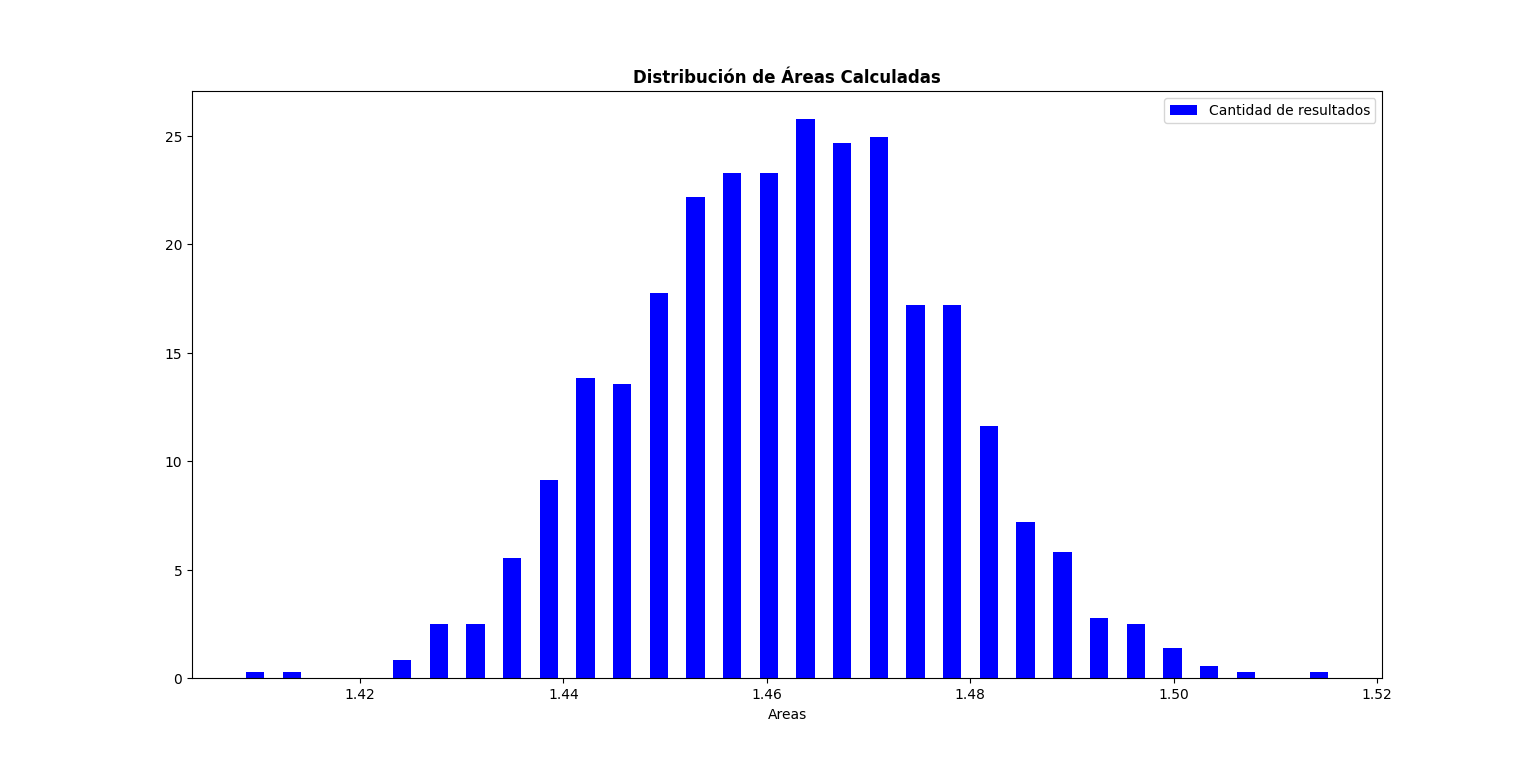
\includegraphics[width=\textwidth]{ejer1.png}
    \end{figure}

    Como se puede ver en la imágen anterior, las barras más altas son 
    las aproximaciónes más certeras de la simulación de Monte Carlo.

    A veces, por los numéros aleatorios tienden a estar a un lado del valor exacto
    de la integral, pero generalmente dan un valor aproximado conforme a la cantidad de 
    intentos que se le da al algoritmo.

    El valor aproximado a la integral es: 1.46579\\
    Con 1000 iteraciones.
    
    \section{Problema 2}
    Calcule:
    \begin{equation}
        I[g(X)] = \int_{-1}^{1} e^{x}4 \,dx
    \end{equation}
    \subsection{Programación}
\begin{lstlisting}
def main():
    a = -1
    b = 1
    f = lambda x: 4*m.e**x
    N = 10000
    calcularArea_MonteCarlo(a,b,f,N)
\end{lstlisting}
    \subsection{Resultados}
    A continuación se muestra la aproximación con la simulación de Monte Carlo y 
    la distribución de los valores dados por el algoritmo y sus frecuencias:
    \begin{figure}[h]
        \centering
        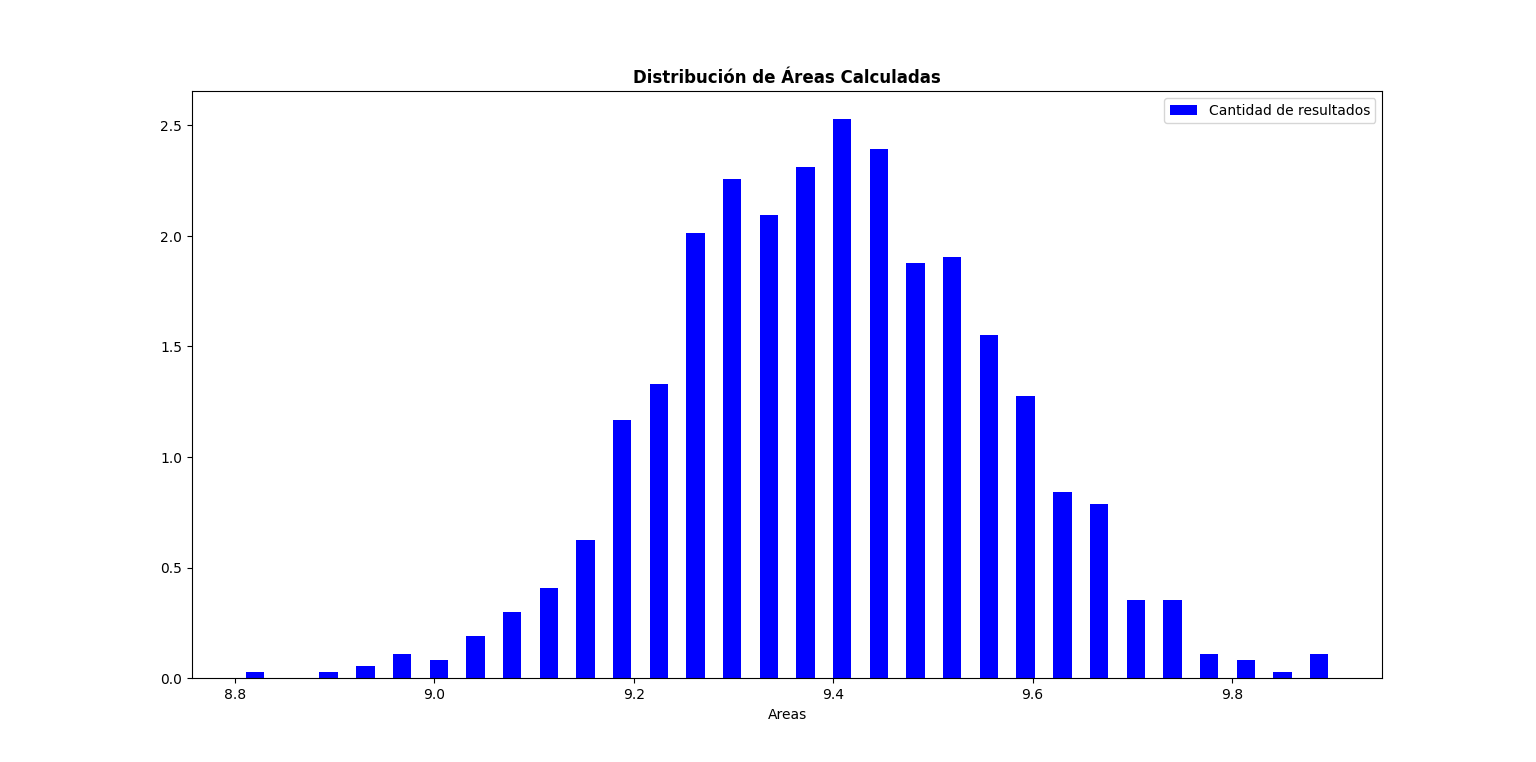
\includegraphics[width=\textwidth]{ejer2.png}
    \end{figure}

    Como se puede ver en la imágen anterior, las barras más altas son 
    las aproximaciónes más certeras de la simulación de Monte Carlo.

    El valor aproximado a la integral es: 9.4138\\
    Que esta muy cerca del valor 9.401(valor más aproximado)\\
    Con 10000 iteraciones.
    \newpage
    \section{Problema 3}
    Calcule:
    \begin{equation}
        I[g(X)] = \int_{0}^{1} (1 - e^2)^{\frac{1}{2}} \,dx
    \end{equation}
    \subsection{Programación****}
\begin{lstlisting}
def main():
    a = 0
    b = 1
    f = lambda x: 1
    N = 1000
    calcularArea_MonteCarlo(a,b,f,N)
\end{lstlisting}
    \subsection{Resultados}
    A continuación se muestra la aproximación con la simulación de Monte Carlo y 
    la distribución de los valores dados por el algoritmo y sus frecuencias:
    \begin{figure}[h]
        \centering
        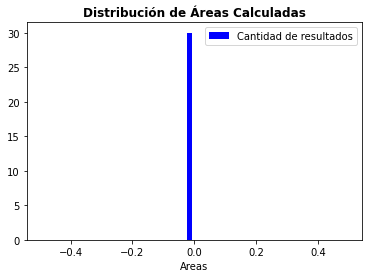
\includegraphics[width=\textwidth]{ejer3_v2.png}
    \end{figure}
    
    En este caso, la distribución de frecuencias dio un valor de 1.
    Esto es porque, \eq{(1-e^2)^{\frac{1}{2}}} es una constante.
    Por lo que:
    \begin{equation}
        (1-e^2)^{\frac{1}{2}} \int_{0}^{1} \,dx
    \end{equation}

    Por lo que el resultado es: \eq{(1-e^2)^{\frac{1}{2}}*[1-0]}

    El valor aproximado a la integral es: 2.527658\ldots\\
    Con 1000 iteraciones.
    \section{Problema 4}
    Calcule:
    \begin{equation}
        I[g(X)] = \int_{0}^{\infty} x(1 + x^2)^{-2} \,dx
    \end{equation}
    \subsection{Programación}
\begin{lstlisting}
def main():
    a = 0
    b = 10000
    f = lambda x: x*((1+x**2)**(-2))
    N = 20000
    calcularArea_MonteCarlo(a,b,f,N)
\end{lstlisting}
\subsection{Resultados}
A continuación se muestra la aproximación con la simulación de Monte Carlo y 
la distribución de los valores dados por el algoritmo y sus frecuencias:
\begin{figure}[h]
    \centering
    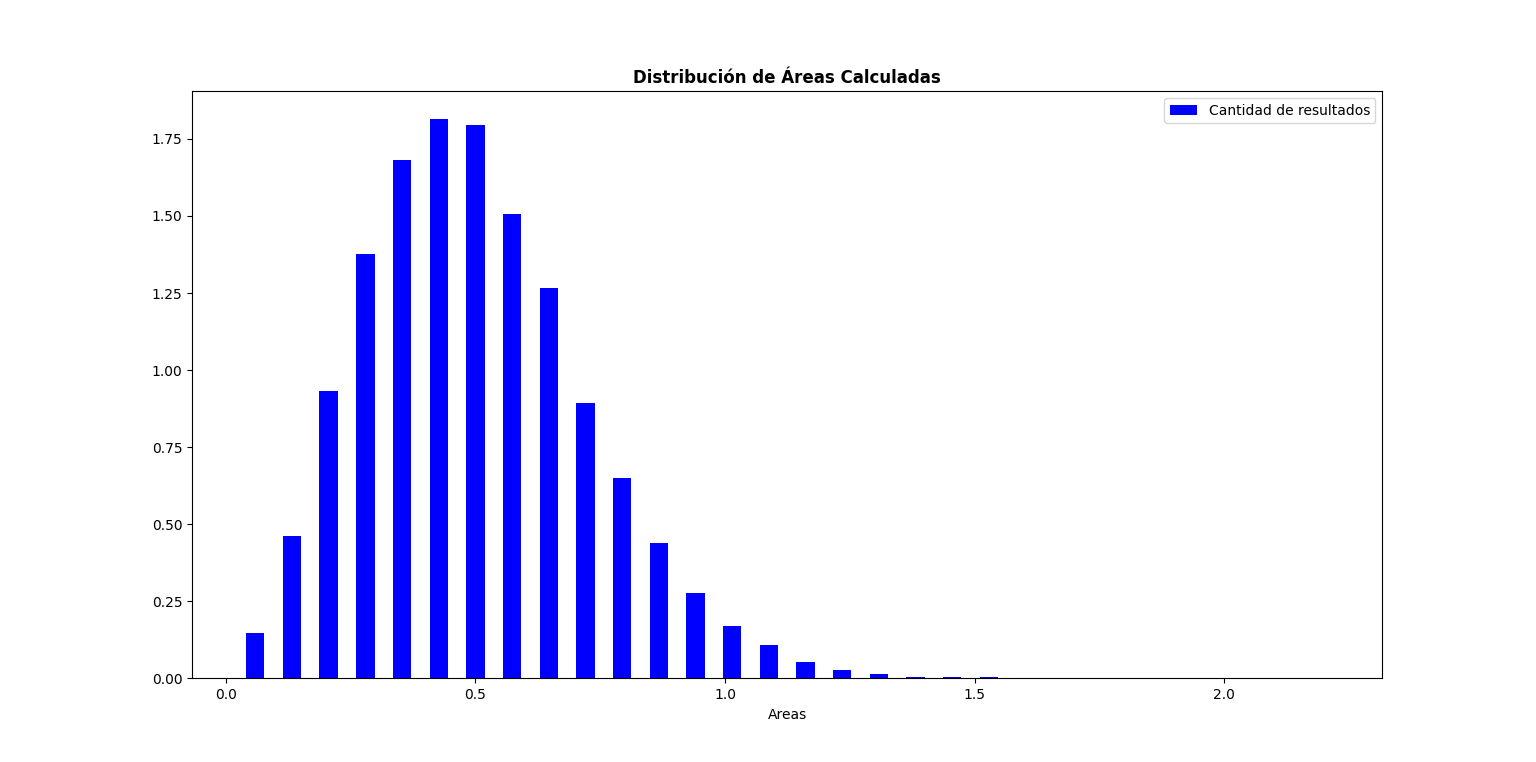
\includegraphics[width=0.8\textwidth]{ejer4.png}
\end{figure}

Como se puede ver en la imágen anterior, las barras más altas son 
las aproximaciónes más certeras de la simulación de Monte Carlo.

El valor aproximado a la integral es: 0.5\\
Con 20000 iteraciones.

\section{Problema 5}
    Calcule:
    \begin{equation}
        I[g(X)] = \int_{0}^{1} e^{x+x^2} \,dx
    \end{equation}
    \subsection{Programación}
\begin{lstlisting}
def main():
    a = 0
    b = 1
    f = lambda x: m.e**(-1*x) 
    N = 10000
    calcularArea_MonteCarlo(a,b,f,N)
\end{lstlisting}

    \subsection{Resultados}
    A continuación se muestra la aproximación con la simulación de Monte Carlo y 
    la distribución de los valores dados por el algoritmo y sus frecuencias:
    \begin{figure}[h]
        \centering
        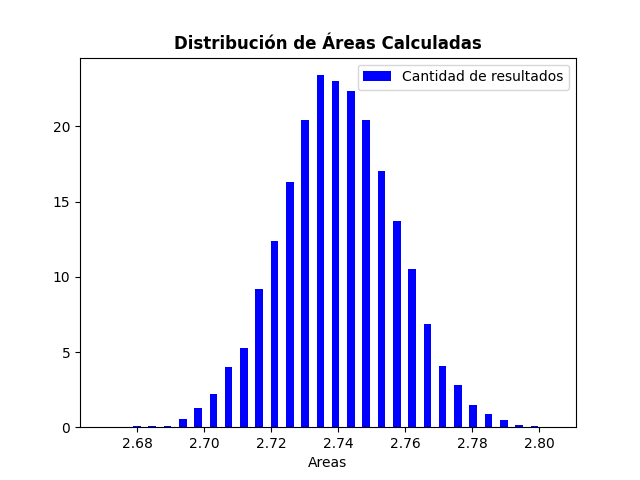
\includegraphics[width=0.8\textwidth]{ejer5.png}
    \end{figure}
    
    Como se puede ver en la imágen anterior, las barras más altas son 
    las aproximaciónes más certeras de la simulación de Monte Carlo.
    
    El valor aproximado a la integral es: 2.7482\\
    Que esta muy próximo de 2.7399(un valor más aproximado a la integral)\\
    Con 10000 iteraciones.

    \section{Problema 6}
    Calcule:
    \begin{equation}
        I[g(X)] = \int_{0}^{\infty} e^{-x} \,dx
    \end{equation}

    \subsection{Programación}
\begin{lstlisting}
def main():
    a = 0
    b = 100000
    f = lambda x: m.e**(-1*x)#x*((1+x**2)**(-2))
    N = 50000
    calcularArea_MonteCarlo(a,b,f,N)
\end{lstlisting}
\subsection{Resultados}
A continuación se muestra la aproximación con la simulación de Monte Carlo y 
la distribución de los valores dados por el algoritmo y sus frecuencias:
\begin{figure}[h]
    \centering
    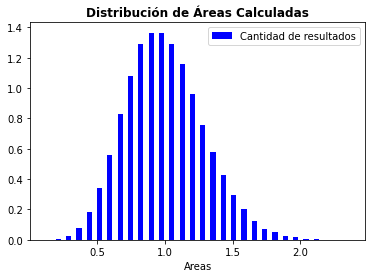
\includegraphics[width=0.8\textwidth]{ejer6.png}
\end{figure}

El valor aproximado a la integral es: 0.91\\
Que esta muy próximo de 1(valor real de la integral)\\
Con 10000 iteraciones.
\section{Anexos}
En el siguiente link se encuentra los archivos de Python:\\
\url{https://drive.google.com/drive/folders/1WiiF428zxfC5vnRzmNjqNCvkJYgYGuyK?usp=sharing}


\end{document}